\documentclass[conference]{IEEEtran}
\IEEEoverridecommandlockouts
\usepackage{cite}
\usepackage{amsmath,amssymb,amsfonts}
\usepackage{algorithmic}
\usepackage{graphicx}
\usepackage{textcomp}
\usepackage{xcolor}
\usepackage{array}
\def\BibTeX{{\rm B\kern-.05em{\sc i\kern-.025em b}\kern-.08em
    T\kern-.1667em\lower.7ex\hbox{E}\kern-.125emX}}

\begin{document}

\title{A Practical AGA-Inspired Selective Synthetic Augmentation Framework for Fine-Grained Bird Classification on CUB-200-2011}

\author{
\IEEEauthorblockN{Author Name}
\IEEEauthorblockA{\textit{Department Name} \\
\textit{University Name}\\
City, Country \\
email@domain.com}
\and
\IEEEauthorblockN{Supervisor Name}
\IEEEauthorblockA{\textit{Department Name} \\
\textit{University Name}\\
City, Country \\
email@domain.com}
}

\maketitle

\begin{abstract}
Fine-grained image classification remains difficult because visually similar classes require highly discriminative supervision, while naively augmenting training data with synthetic images can introduce substantial noise. This paper studies a practical AGA-inspired synthetic augmentation pipeline for CUB-200-2011 in which generated bird images are not accepted blindly but filtered through a selective sample-admission process. The implemented framework combines class-consistency scoring, CLIP-based semantic filtering, DINO-based diversity pruning, class-balance control, and optional attribute-aware coverage. In the saved experimental results, selective synthetic augmentation improved test accuracy from 0.1388 in a real-only baseline to 0.1505, while naive real-plus-all-synthetic augmentation reached 0.1367. The ablation results support the broader claim that synthetic sample selection matters, while also showing that the more complex filtering stack did not outperform confidence-only selection in the saved run. Because the evaluation was conducted under constrained compute and the full multi-seed benchmark package is still incomplete, the present evidence should be interpreted as preliminary but reproducible rather than as an exhaustive benchmark study.
\end{abstract}

\begin{IEEEkeywords}
fine-grained classification, synthetic augmentation, CLIP, DINO, CUB-200-2011, empirical study
\end{IEEEkeywords}

\section{Introduction}
Fine-grained visual classification is challenging because classes often differ by subtle local cues, pose, texture, and part structure rather than by broad object shape alone. In bird recognition datasets such as CUB-200-2011, small appearance variations and strong background bias make the learning problem especially difficult. Synthetic augmentation is an appealing strategy for increasing data diversity, but adding all generated samples without verification can degrade the training signal rather than improve it.

This work studies a practical and reproducible alternative: generated candidates are passed through a selective admission process before they are added to the final training set. The key idea is that not every generated image is equally useful for downstream recognition. Instead of rewarding synthetic quantity, the proposed pipeline rewards synthetic quality. The method is intentionally described as \emph{AGA-inspired} rather than as an exact reproduction of Automated Generative Data Augmentation (AGA), because the implemented generation stage is a practical foreground-preserving approximation rather than a matched reimplementation of the original upstream method.

The main contribution of this paper is not a claim of state-of-the-art performance. The contribution is a selective synthetic augmentation workflow that is fully implemented, reproducible, and empirically evaluated on CUB-200-2011. Under the saved run in this repository, selected synthetic augmentation outperformed both the real-only baseline and a naive real-plus-all-synthetic setting. The current evidence therefore supports a careful empirical claim: synthetic selection quality mattered more than synthetic quantity in the evaluated setup.

\section{Related Work}
Fine-grained recognition on CUB-200-2011 has been widely used to study subtle visual discrimination and dataset-specific challenges such as pose, background bias, and part-level variation \cite{wah2011}. More recent work has explored the use of generative models and synthetic augmentation to improve image classification, including practical efforts to incorporate generated samples into downstream supervised training pipelines \cite{rahat2025}.

Large vision-language models such as CLIP provide a useful way to score semantic agreement between an image and its intended class text, making them attractive for filtering noisy synthetic samples \cite{radford2021}. Self-supervised visual encoders such as DINO have also shown strong representation quality for measuring similarity and diversity among images \cite{caron2021}. This paper combines these ideas in a single sample-admission pipeline, but the current evidence suggests that the overall selective framework is more strongly supported than any claim about the necessity of each individual module.

\section{Method}
\subsection{Dataset and Split}
All experiments use the CUB-200-2011 dataset \cite{wah2011}. In the prepared repository split, the dataset contains 11,788 images across 200 classes, with 5,394 training images, 600 validation images, and 5,794 test images. Optional image-level attribute metadata from CUB is retained as auxiliary information for the attribute-aware coverage variant.

\subsection{AGA-Inspired Candidate Generation}
The generation stage is implemented as a foreground-preserving augmentation pipeline rather than as a strict reimplementation of the base AGA method. Bird foregrounds are preserved using available dataset structure, while context and appearance are perturbed to create candidate synthetic images. This design keeps the project reproducible inside a constrained environment while still producing a large candidate pool for downstream filtering.

\subsection{Selective Sample Admission}
The proposed admission pipeline evaluates synthetic candidates using four main signals.
\begin{itemize}
\item Class-consistency confidence from the baseline classifier
\item CLIP semantic alignment to the intended bird class
\item DINO diversity pruning to reduce redundancy
\item Class-balance control, with an optional attribute-aware coverage variant
\end{itemize}

The final selected set is intentionally small. In the saved run, 400 synthetic candidates were generated and only 15 were retained after filtering, corresponding to a selection rate of 3.75\%. This aggressive filtering is central to the paper's empirical story.

\subsection{Training Protocol}
The repository includes three main experiments:
\begin{itemize}
\item \texttt{exp1\_real\_only}: supervised training on real images only
\item \texttt{exp2\_real\_plus\_all\_synthetic}: training with all synthetic candidates
\item \texttt{exp3\_real\_plus\_selected\_synthetic}: training with only the selected synthetic subset
\end{itemize}

The saved experiments use a ResNet-18 backbone with 224 pixel inputs, 30 epochs, patience 7, batch size 32, learning rate 0.0003, weight decay 0.0001, and label smoothing 0.1. The current paper is based on the saved repository outputs rather than on a completed multi-seed benchmark package.

\section{Experimental Evidence}
\subsection{Main Results}
Table \ref{tab:main_results} summarizes the saved main experiment results. The selected-synthetic configuration achieved the highest test accuracy among the three main settings.

\begin{table}[htbp]
\caption{Saved main experiment results from the current repository outputs.}
\label{tab:main_results}
\begin{center}
\begin{tabular}{|p{3.1cm}|c|c|}
\hline
\textbf{Experiment} & \textbf{Test Accuracy} & \textbf{Macro-F1} \\
\hline
Real-only baseline & 0.1388 & 0.1111 \\
\hline
Real + all synthetic & 0.1367 & 0.1025 \\
\hline
Real + selected synthetic & 0.1505 & 0.1206 \\
\hline
\end{tabular}
\end{center}
\end{table}

The results support two practical observations. First, adding all synthetic samples did not improve performance in the saved run. Second, selective synthetic augmentation improved over both internal controls under the same overall training setup.

\subsection{Ablation Results}
Table \ref{tab:ablation_results} reports the saved ablation results. The strongest saved result came from confidence-only filtering, while the more complex variants produced the same lower accuracy in the current run.

\begin{table}[htbp]
\caption{Saved ablation results from the current repository outputs.}
\label{tab:ablation_results}
\begin{center}
\begin{tabular}{|p{4.2cm}|c|}
\hline
\textbf{Ablation Variant} & \textbf{Test Accuracy} \\
\hline
Confidence only & 0.1555 \\
\hline
Confidence + CLIP & 0.1505 \\
\hline
Confidence + CLIP + DINO & 0.1505 \\
\hline
Confidence + CLIP + DINO + balance & 0.1505 \\
\hline
Confidence + CLIP + DINO + balance + attribute coverage & 0.1505 \\
\hline
\end{tabular}
\end{center}
\end{table}

These ablations support the selective-admission idea, but they do not support a strong claim that all additional filtering stages improved over confidence-only selection.

\subsection{Selection Statistics}
The selection statistics further justify the paper's central claim. Out of 400 synthetic candidates, 15 were retained and 385 were rejected. The mean combined score of the selected pool was 0.2285, and the mean CLIP score was 0.3361. DINO pruning did not remove any samples under the saved threshold of 0.96, so the current run does not demonstrate a measurable DINO benefit.

\section{Qualitative Evidence}
Fig. \ref{fig:candidates} shows representative synthetic candidates from the generation stage. Fig. \ref{fig:accepted_rejected} contrasts accepted and rejected synthetic examples, illustrating the qualitative purpose of the selection module. Fig. \ref{fig:main_plot} summarizes the main experiment comparison, and Fig. \ref{fig:ablation_plot} visualizes the ablation study.

\begin{figure}[htbp]
\centerline{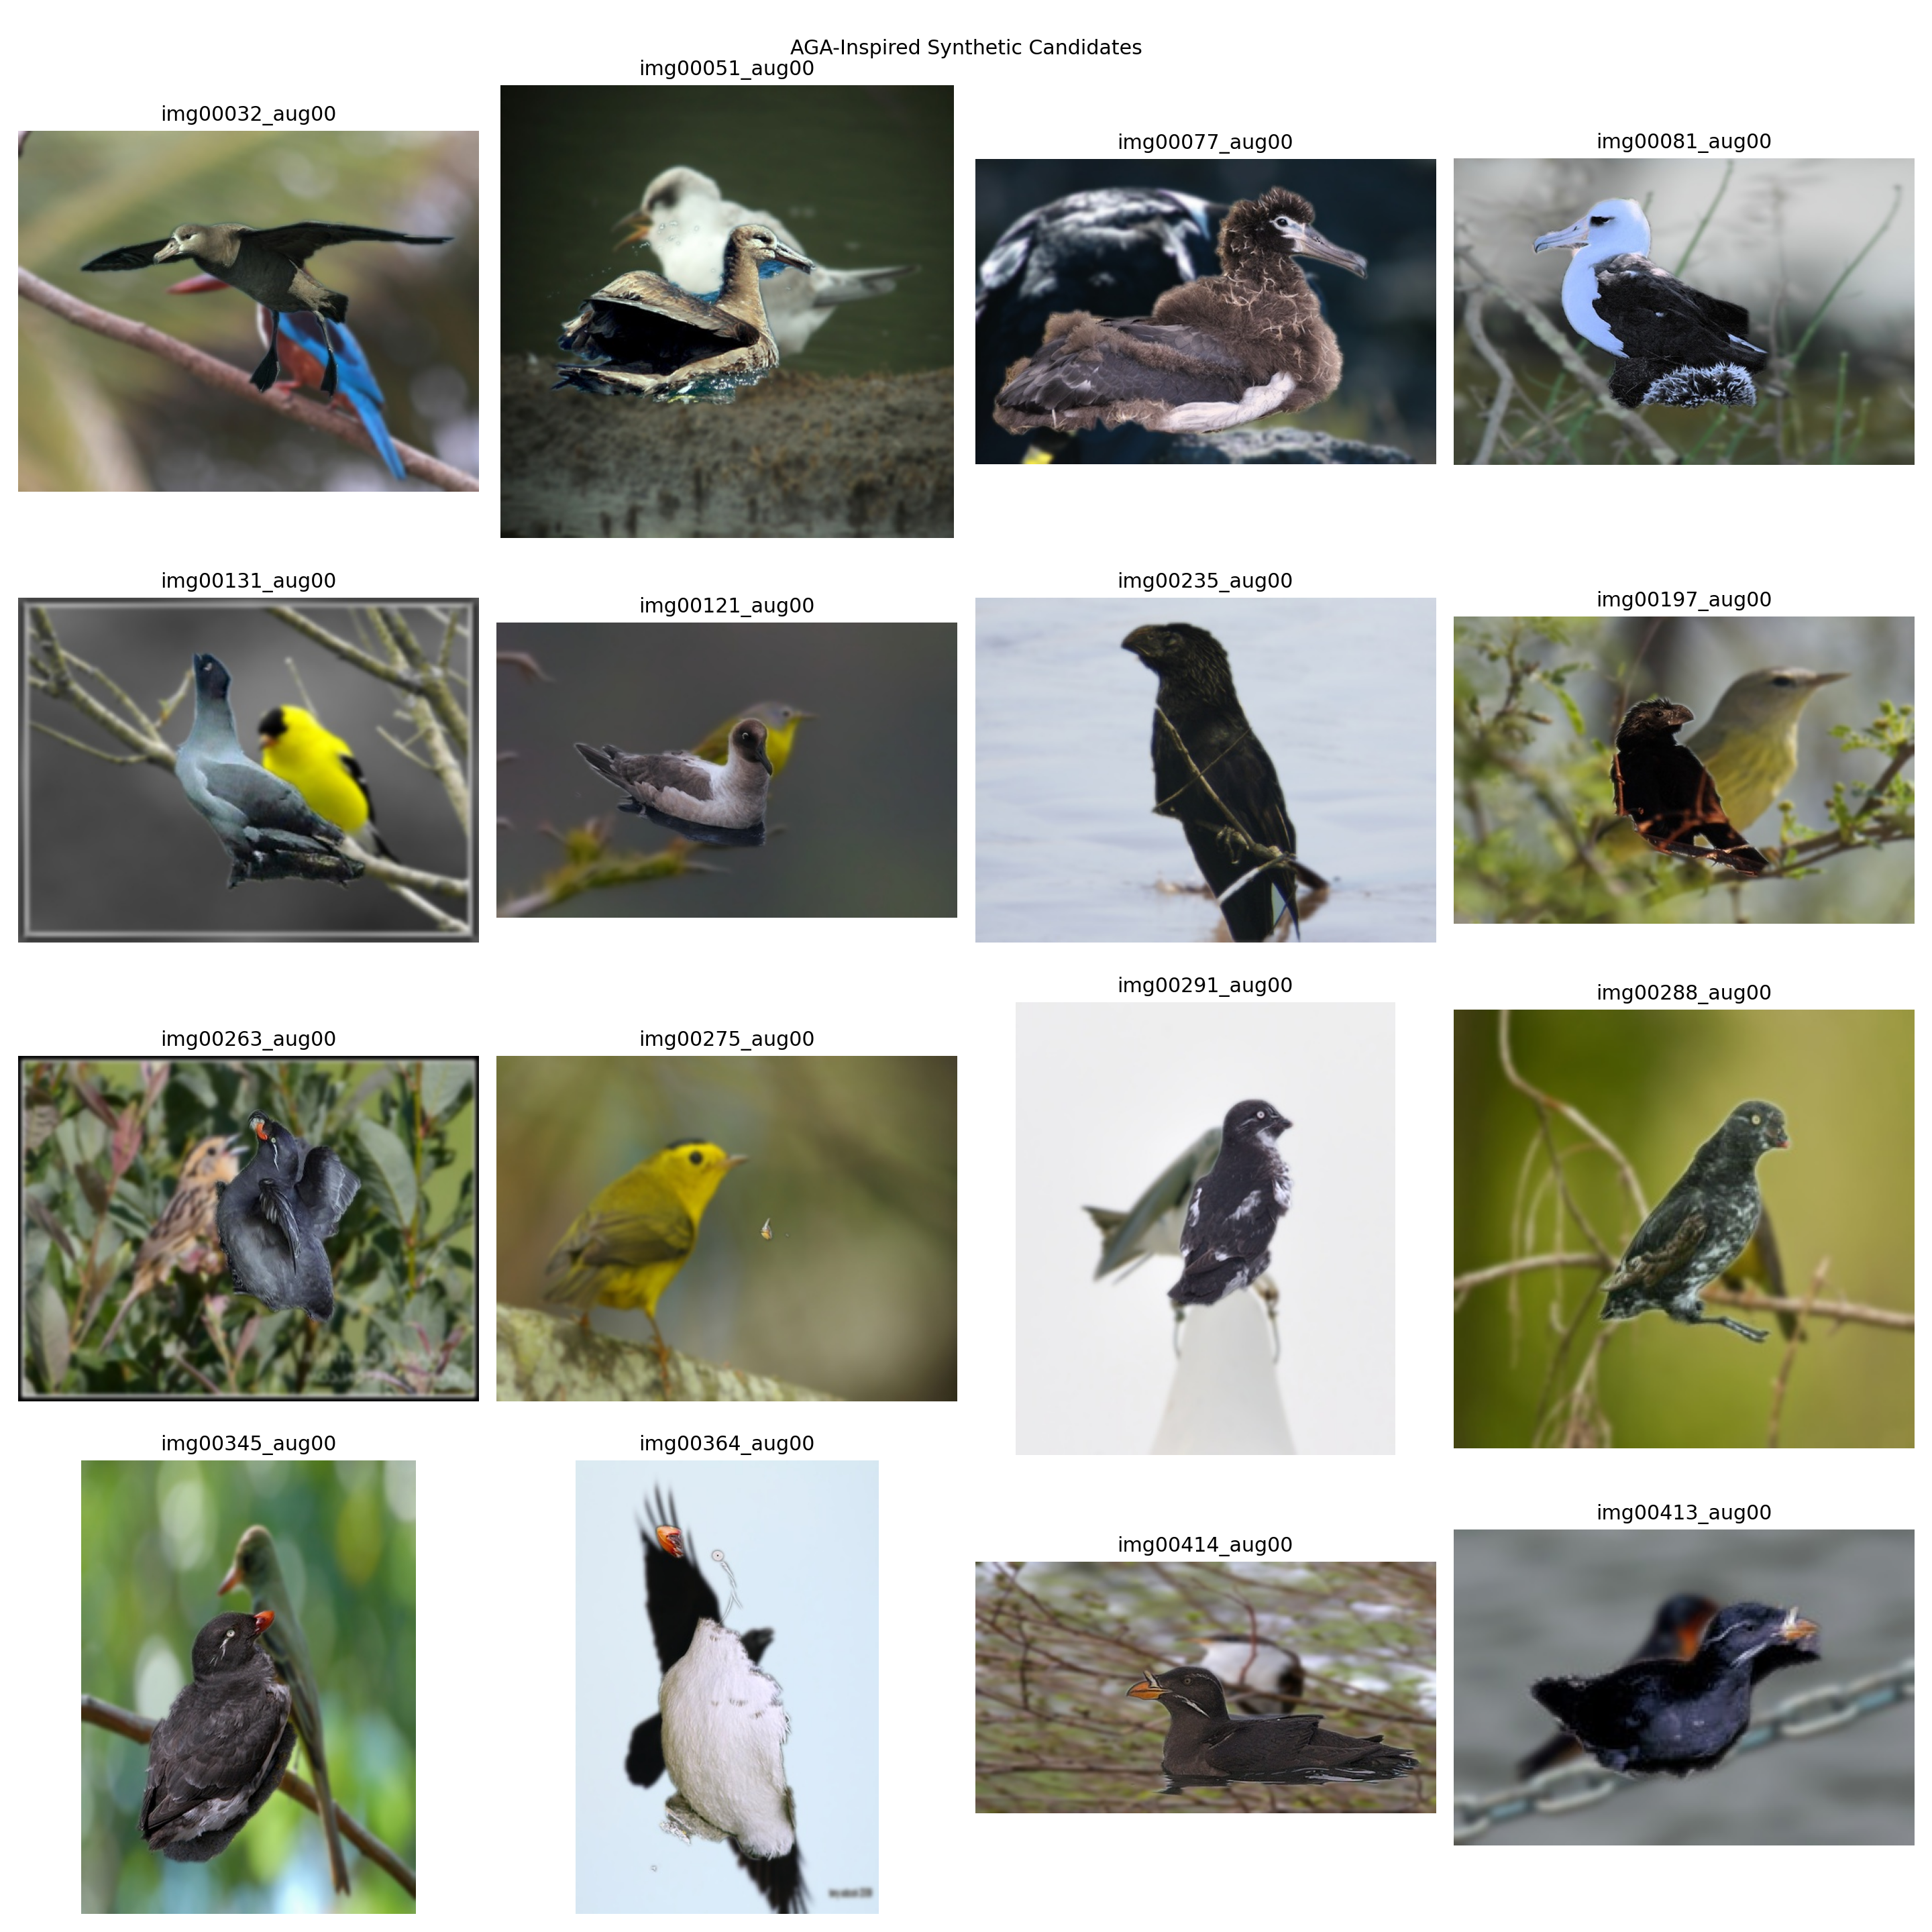
\includegraphics[width=0.48\textwidth]{../outputs/samples/synthetic_candidate_grid.png}}
\caption{Synthetic candidate examples produced by the AGA-inspired generation pipeline.}
\label{fig:candidates}
\end{figure}

\begin{figure}[htbp]
\centerline{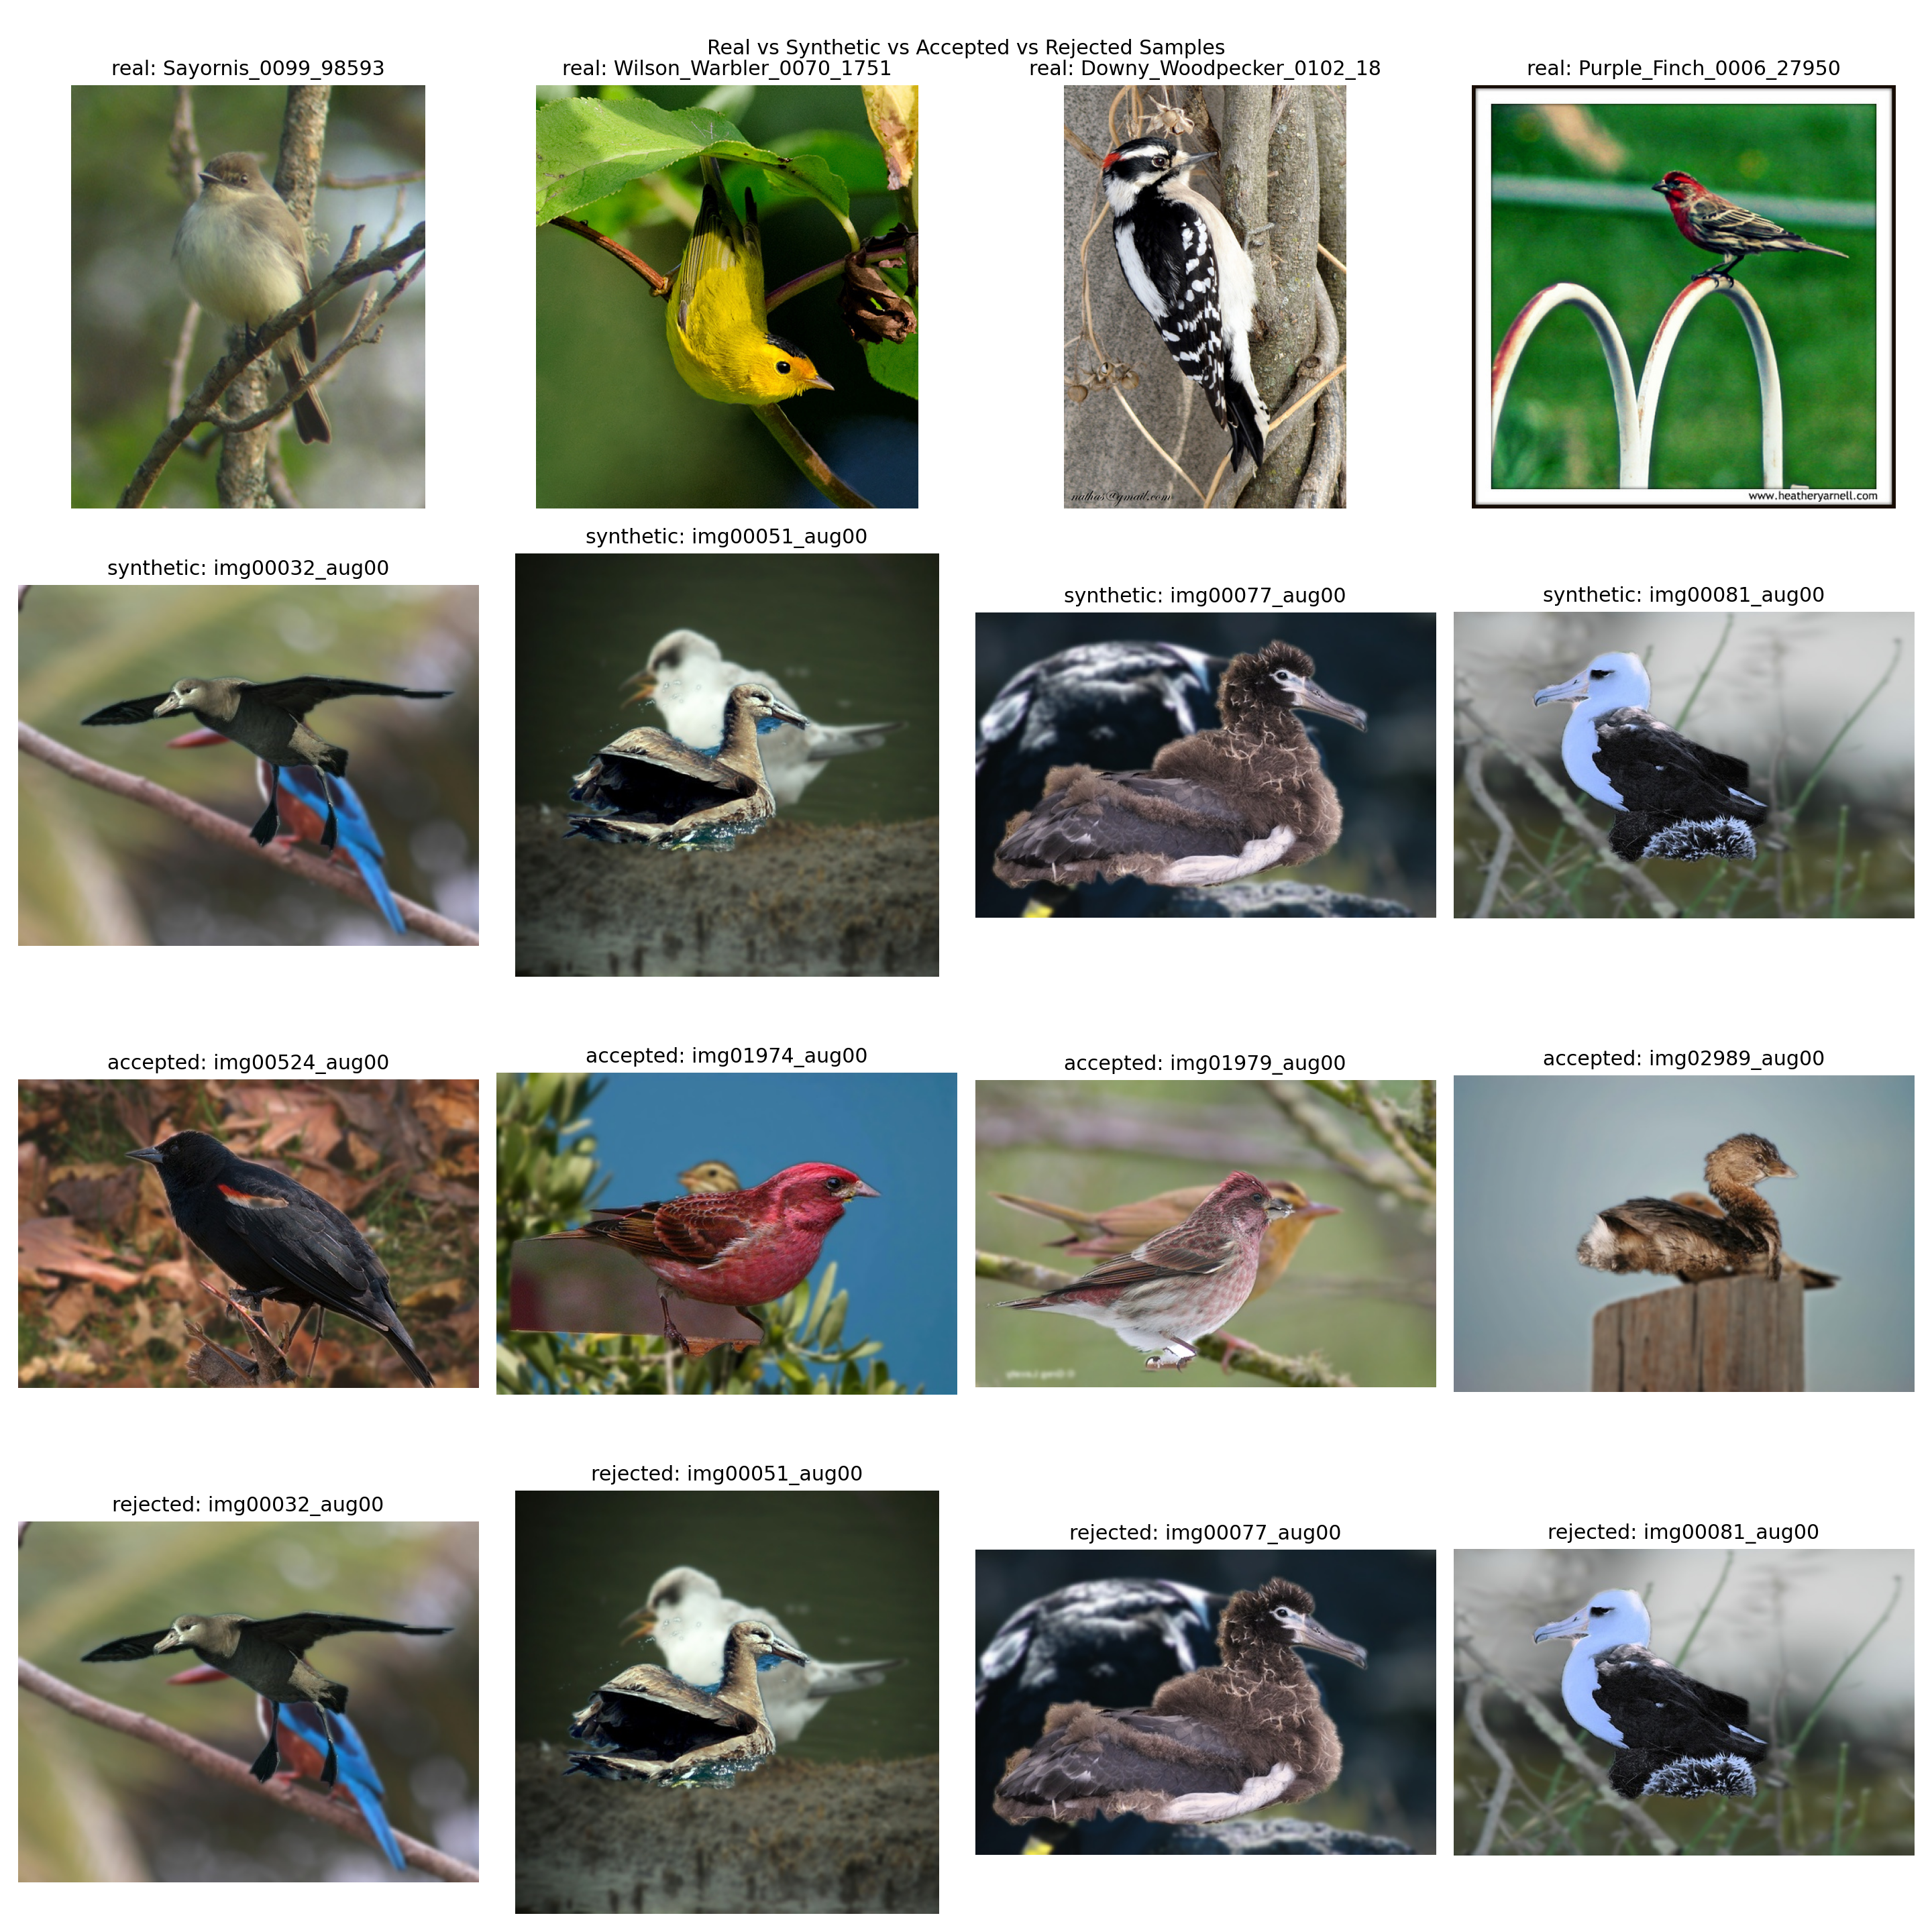
\includegraphics[width=0.48\textwidth]{../outputs/samples/real_vs_synthetic_vs_accepted_vs_rejected_grid.png}}
\caption{Qualitative comparison of real, synthetic, accepted, and rejected samples.}
\label{fig:accepted_rejected}
\end{figure}

\begin{figure}[htbp]
\centerline{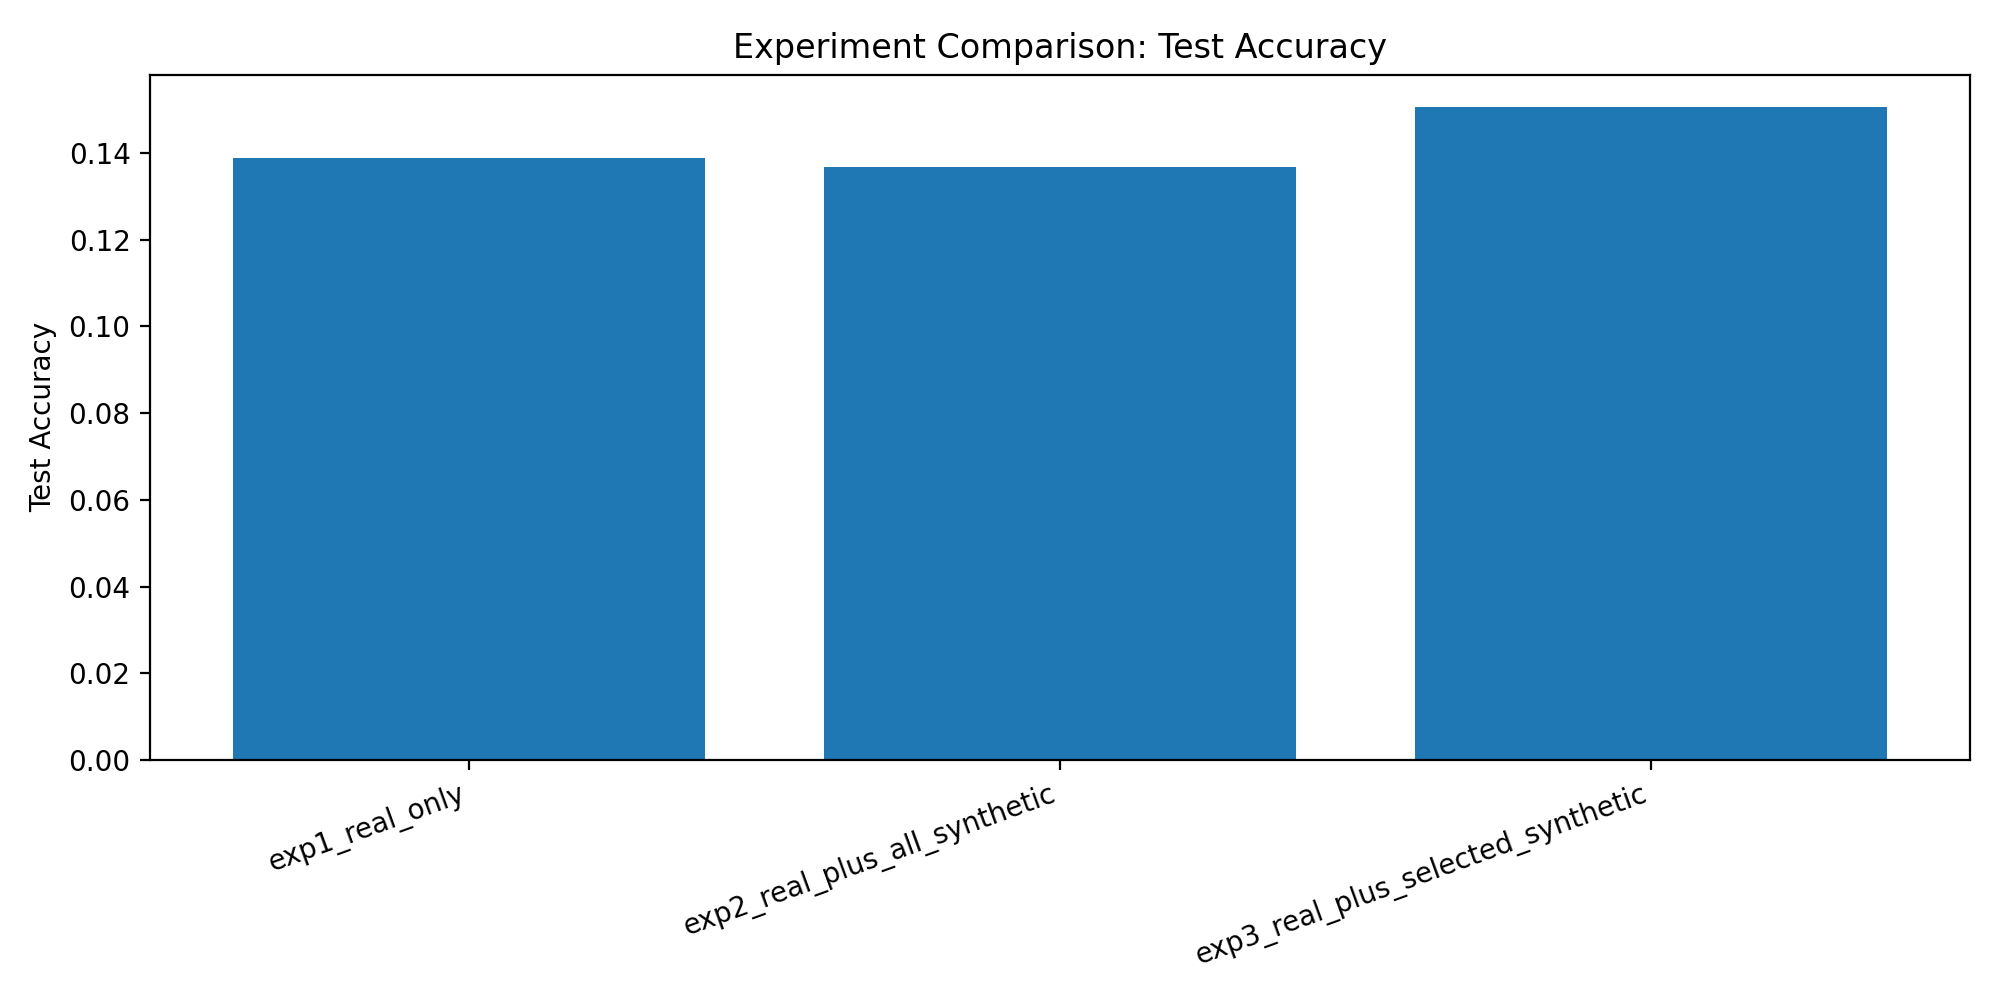
\includegraphics[width=0.48\textwidth]{../outputs/plots/experiment_comparison_accuracy.png}}
\caption{Accuracy comparison across the three main experiments.}
\label{fig:main_plot}
\end{figure}

\begin{figure}[htbp]
\centerline{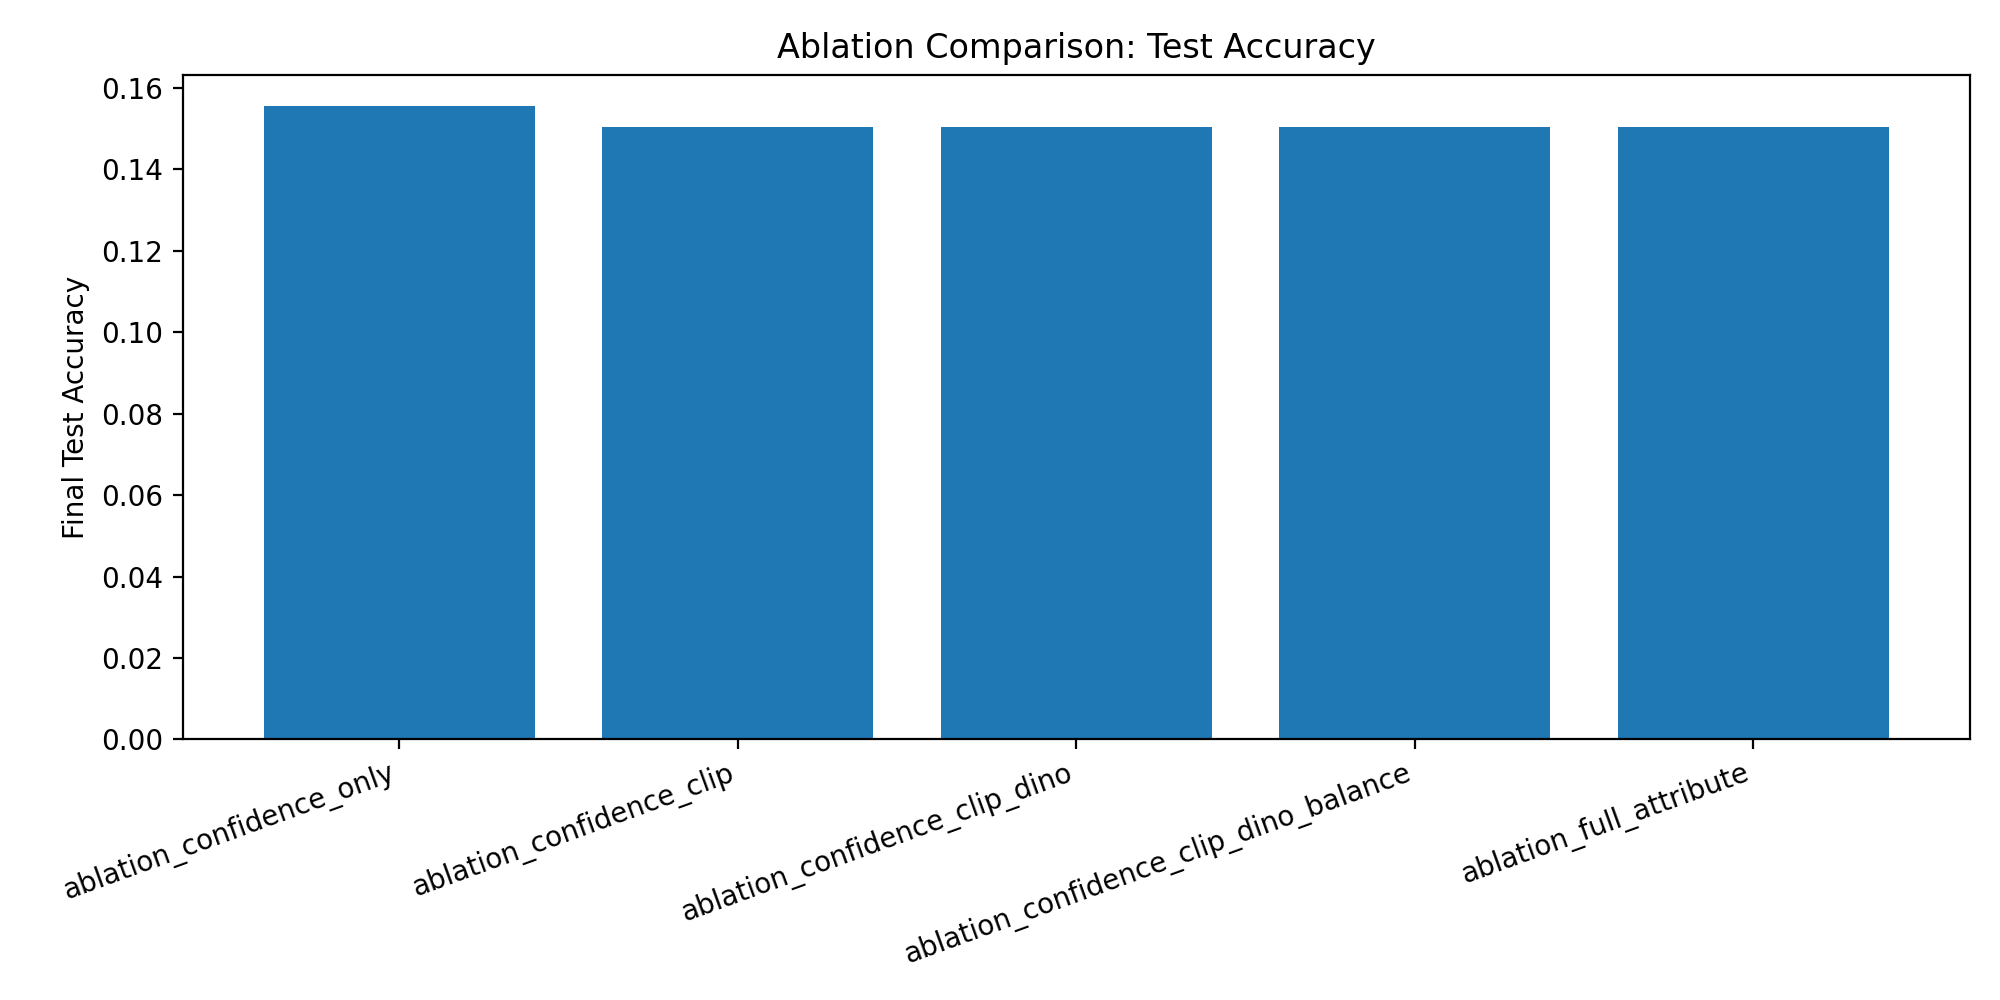
\includegraphics[width=0.48\textwidth]{../outputs/plots/ablation_comparison_accuracy.png}}
\caption{Ablation comparison across the selection variants.}
\label{fig:ablation_plot}
\end{figure}

\section{Discussion}
The current evidence supports a narrow but useful conclusion. In this setup, blindly adding synthetic data was not beneficial, but filtering synthetic data before final training was beneficial. This finding is practically relevant because it suggests that synthetic augmentation pipelines should invest more effort in admission quality than in candidate quantity.

At the same time, the current ablation results caution against overclaiming. The broader selective-admission framework is supported, but the individual roles of CLIP, DINO, class-balance control, and attribute-aware coverage are not equally justified by the present saved run. In particular, the DINO pruning stage did not remove any samples under the stored threshold, and the full filtering stack did not surpass confidence-only filtering.

\section{Limitations}
This study has four important limitations. First, the generation stage is AGA-inspired rather than an exact reproduction of the original AGA paper. Second, the strongest current evidence comes from saved single-run outputs rather than from a completed multi-seed benchmark package. Third, the experiments were conducted under compute and environment constraints, which limited the scale of repeated training. Fourth, the base-paper comparison file in the repository does not currently support a fair claim of improvement over the WACV 2025 method.

These limitations do not invalidate the paper's empirical contribution, but they do narrow the claims that can be made responsibly. The paper should therefore be positioned as a reproducible empirical study under constrained compute rather than as a definitive benchmark paper.

\section{Conclusion}
This paper presented a practical AGA-inspired selective synthetic augmentation framework for fine-grained bird classification on CUB-200-2011. Under the saved repository results, selected synthetic augmentation outperformed both a real-only baseline and a naive all-synthetic condition, supporting the central claim that synthetic sample quality mattered more than synthetic quantity in the tested setup. The evidence also showed that the broader selective-admission idea is more strongly justified than any claim about the necessity of every added filtering module. With careful wording, explicit limitations, and a reproducible repository, this work forms a defensible IEEE-style empirical paper and a strong project-level research submission.

\begin{thebibliography}{00}
\bibitem{wah2011} C. Wah, S. Branson, P. Welinder, P. Perona, and S. Belongie, ``The Caltech-UCSD Birds-200-2011 Dataset,'' California Institute of Technology, Tech. Rep. CNS-TR-2011-001, 2011.
\bibitem{radford2021} A. Radford et al., ``Learning transferable visual models from natural language supervision,'' in \emph{Proc. ICML}, 2021, pp. 8748--8763.
\bibitem{caron2021} M. Caron et al., ``Emerging properties in self-supervised vision transformers,'' in \emph{Proc. ICCV}, 2021, pp. 9650--9660.
\bibitem{rahat2025} A. Rahat, M. A. B. S. Nahin, and M. R. Amin, ``Data augmentation for image classification using generative AI,'' in \emph{Proc. WACV}, 2025.
\bibitem{cubsite} Caltech, ``CUB-200-2011 Dataset,'' Available: https://www.vision.caltech.edu/datasets/cub\_200\_2011/. Accessed: Apr. 25, 2026.
\end{thebibliography}

\end{document}
